\subsection{Implementierung des Release-Management-Prozesses}

Der Release-Management-Prozess enthält alle notwendigen Schritte, bis die Software auf das Endprodukt verteilt wird. Dies sind die Entwicklung-,Build-,Test- und Deployment-Phase. Sobald der Entwicklungsprozess abgeschlossen ist, erfolgt die automatischen weiteren Phasen wie Build-, Release- und Deployment-Phase. Das Update kann sowohl für alle angeschlossenen Ampelanlagen als auch für verschiedene Ampelanlagen durchgeführt werden. 
\newline\newline
Im Laufe dieses Kapitels wird den ausgewählten Entwicklungsprozessentwurf umgesetzt und wird darauf eingegangen, wie es in der Realität ein Release erstellt wird.
In der Buildphase wird die benötigte Dateien und deren Abhängigkeiten übersetzt und das Ergebnis zur Verfügung gestellt. Diese Phase ist für den gesamten Entwurf und die Implementierung der Architektur erforderlich. Nach der Build- und Release-Phase erfolgt die Deployment-Phase. In dieser Phase wird die Übertragung der Software bis zum Ampelanlage geschehen. Die Ausführung der Phasen erfolgt so weit wie möglich automatisiert und falls während der Ausführung Fehler auftreten, wird die Pipeline unterbrochen, wodurch die Fortsetzung der anderen Phasen verhindert wird.

\subsubsection{Umsetzung der Continues Integration und Continues Delivery Methode}

Nun nach der Entwicklungsphase kommt die \ac{CD}-Phase zustande. Nach dem Start der \ac{CD}-Pipeline beginnt die kontinuierliche Deployment-Phase an. Zu \ac{CD} gehört die Build-,Release- und die Deployment-Phase. Um Continues Integration und Continues Delivery mit GitLab nutzen zu können, wird einen GitLab Runner benötigt. GitLab Runner ist eine Build-Instanz, die verwendet wird, um Aufgaben auf mehreren Computern auszuführen und die Ergebnisse durch „artifacts“ an GitLab zu übertragen.
\newline\newline
In diesem Projekt wird der Gitlab Runner auf dem Master-Node konfiguriert und mit einem Executer vorgesehen, der die vordefinierten Aufgaben in Gitlab aus-
führt. Sobald der Runner registriert ist, initiiert das Runner Tag die Kommunikation zwischen der Gitlab-Plattform und dem Master-Node, auf dem der Runner installiert ist. Die möglichen Executors sind beispielsweise SSH, Shell, Docker, Kubernetes und einige andere. In diesem Projekt wird Kubernetes-Executer benutzt.
\newline\newline
Im
Folgenden werden die einzelnen Phasendurchführungen erklärt.
\subsubsection*{Build-Phase}

Nun wenn die Pipeline gestartet wird, beginnt die Phasendurchführung der \ac{CI}. Die erste \ac{CI}-Phase ist die Build-Phase, da in diesem Projekt Programmiersprache Python verwendet wird, wird diese Phase nicht in der Pipeline-Stages hinzugefügt.

\subsubsection*{Test-Phase}

Nachdem der Prozess Merge von \textit{develop} Branch mit \textit{main} Branch gestartet wird, beginnt die \ac{CI}-Testphase. Für die Testphase wird die Master-Node verwendet. In diesem Projekt wird Unit-Test für den RaspberryPi GPIO ausgeführt. Der Erfolg des Merge-Prozesses hängt von den Ergebnissen von Unit-Test ab. Wenn der Test nicht erfolgreich abgeschlossen werden kann, wird auch der Merge-Prozess abgebrochen, um eine weitere Ausführung der \ac{CD}-Phasen zu verhindern.

\subsubsection*{Release Phase}

Nach erfolgreichem Merge-Prozess kann die weitere \ac{CI/CD}-Phase fortgesetzt werden. Nach der Vergabe des Release-Tags wird die Pipeline gestartet und die zweite Pipeline-Stage dieses Projektes ist die \glqq Publish and Release Phase\grqq. In dieser Phase wird die entwickelte Software als Docker-Image gekapselt, auf die Dockerhub-Plattform hochgeladen und zur Übertragung und/oder Installation bereitgestellt. Für die Ausführung dieser Phase wird erneuert der Runner der Master-Node benötigt. Durch das Hochladen des Images wird einen neuen Release erstellt. Außerdem wird ein gewohnliche Release auf dem GitLab-Plattform erstellt. Die Abbildung~\ref{fig:release-stage} veranschaulicht die Release-Phase anhand eines Sequenzdiagramm.


\begin{figure}[bth] 
	\centering
	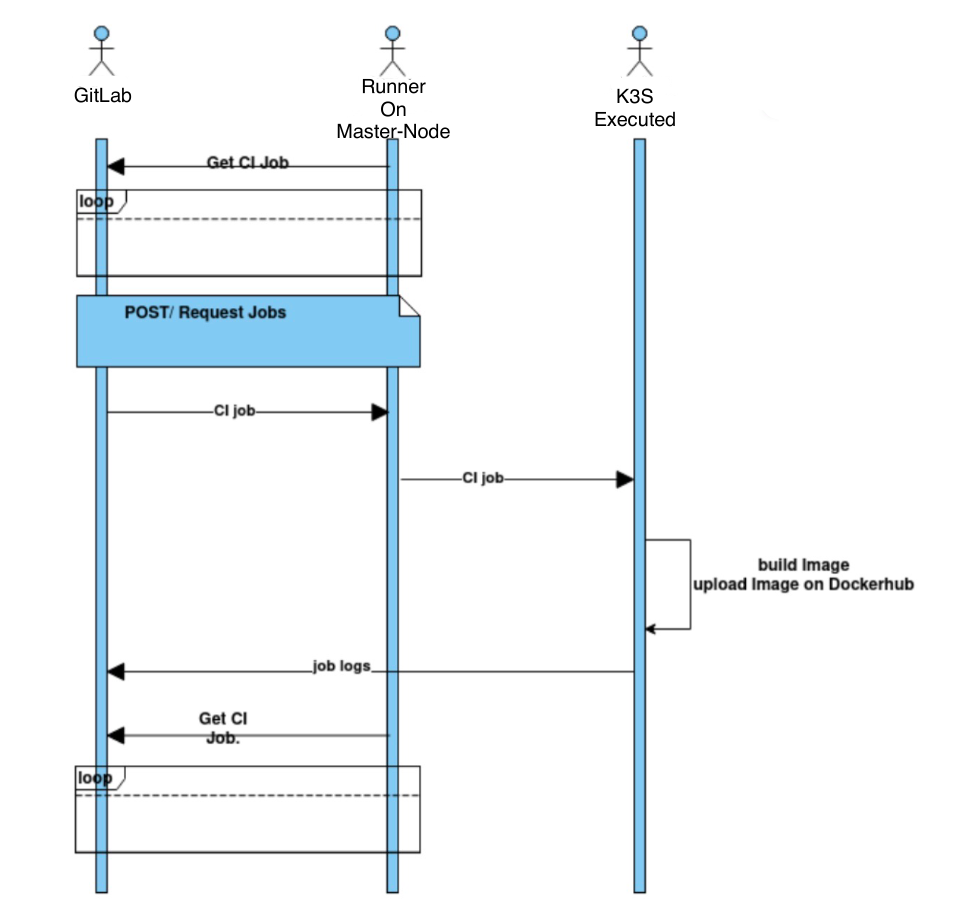
\includegraphics[width=0.9\textwidth]{Graphics/release.png}
	\caption{Publish on Docker Hub}
	\label{fig:release-stage}
\end{figure}


\subsubsection*{Deployment-Preparation Stage}

Die Deployment-Phase besteht aus Preparation- und Deployment-Stage. In der CI-Datei nach Release-Stage folgt preparation Stage. Wie Build und Release-Stage verwendet diese Stage denselben registrierten Runner, die auf dem Master-Node gezielt ausgeführt wird. Normalerweise verteilt die Kubernetes-Technologie die Masterlast auf die wenig belasteten Worker-Nodes. In dieser Architektur wird diese Eigenschaft jedoch aufgegeben, um die Verteilung der Arbeit auf die Nodes vollständig zu steuern. Wie in der Abbildung~\ref{fig:rigister-temp-runner} gezeigt, werden die zu erstellenden Runner gemäß den eingegebenen Zielen beschriftet (eng. Label).
\newline\newline
Preparation-Stage ist für die dynamische Erstellung von Deployment-Stages verantwortlich, abhängig von der Zieleingabe. Daher können Entwickler entscheiden, welche Software auf welcher Ampelanlage übertragen wird. In GitLab kann diese Anforderung durch eine „Subpipeline“ erfüllt werden, sodass die CI-Datei dynamisch zusätzliche YAML-Datei erstellt und diese mit dem Schlüsselwort „trigger“ in Deployment-Stage einbindet. Diese dynamische YAML-Datei basierend auf der RaspberryPi-Anzahl bzw. Worker-Node-Anzahl werden mit einem Shell-Skript erstellt. Dieses Skript ist auch dafür verantwortlich, das Label des Runners in dieser Datei einzutragen. Die Erstellung einer Pipeline mit dem gewünschten Ziel-Raspberry Pi wird anhand dieses Labels in der Deployment-Stage erreicht. Die Einbindung geschieht durch das Schlüsselwort “include „ und die erstellte Dateien werden mithilfe von \glqq \textit{artifacts}\grqq auf andere Ebenen bzw. Stages übertragen.


\begin{figure}[bth] 
	\centering
	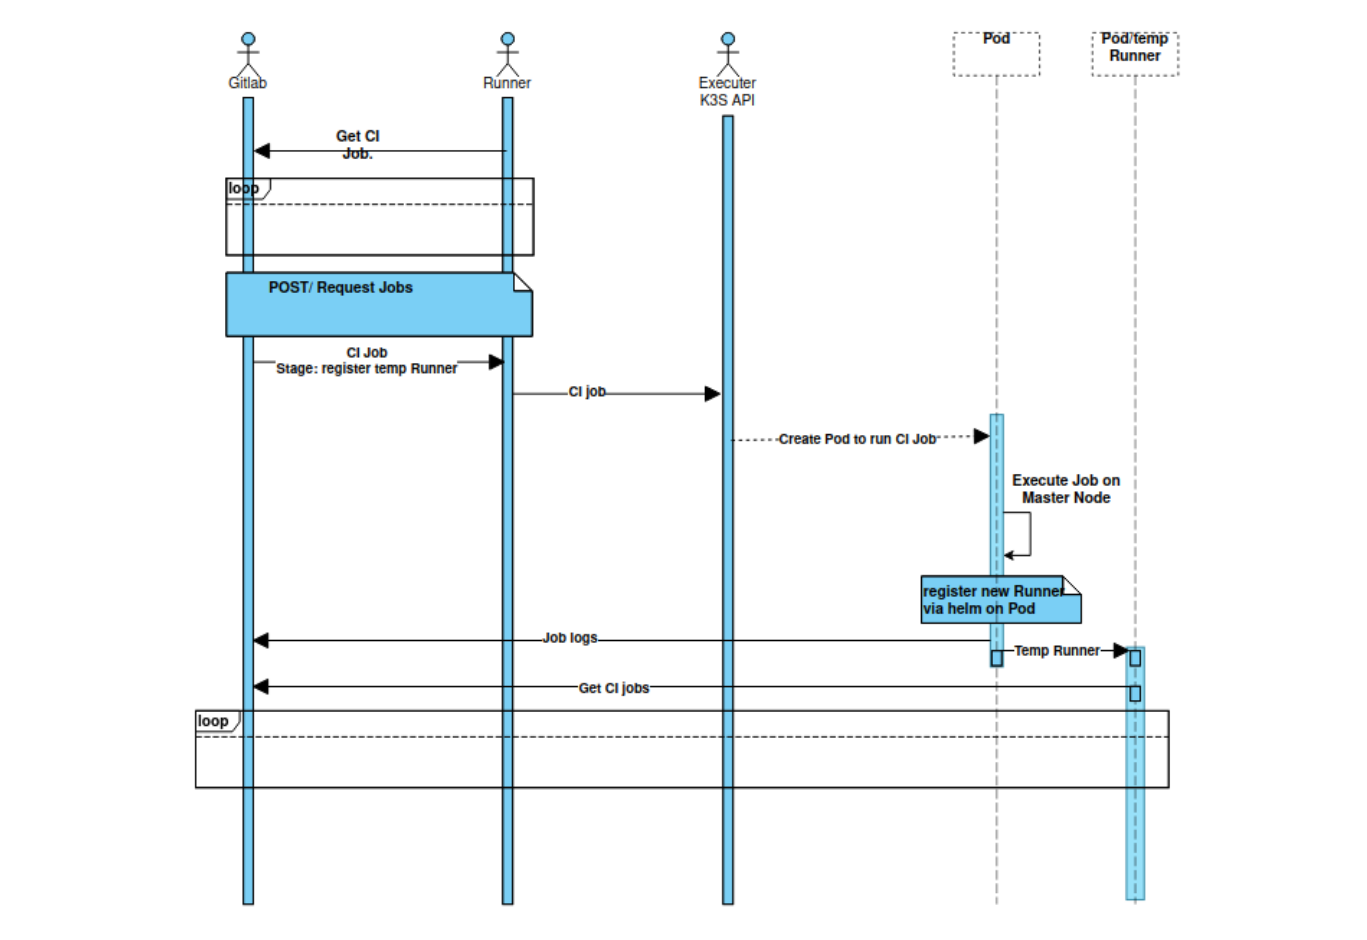
\includegraphics[width=0.9\textwidth]{Graphics/register-temp-runner.png}
	\caption{Die Registrierung eines Runners auf Master-Node mithilfe von Helm-Tool}
	\label{fig:rigister-temp-runner}
\end{figure}



\subsubsection*{Deployment Stage}

Nachdem die YAML-Datei dynamisch für die Übertragung erstellt wurden, wird die Software automatisch direkt auf den benötigten Raspberry Pi übertragen. Um dies zu ermöglichen, wird an dieser Stelle die Datei “triger-child-pipeline.yaml „ wie oben bereits erwähnt über Trigger aufgerufen und dies führt zum Start der Child-Pipelines der Ziel-RaspberryPis. Jede Child-Pipeline überträgt die ihr zugewiesene Informationen unabhängig von den anderen Child-Pipelines auf ihren Ziel-Raspberry Pi durch den Master-Node und der Fortschritt der Arbeit wird auf GitLab angezeigt. Die Software wird als Docker-Image aus dem DockerRepository heruntergeladen und ausgeführt. Der gestartete Docker Container stellt sicher, dass eine korrekte Umgebung für die Ausführung eines Python-Skripts eingestellt ist.

\subsubsection*{Clean-Stage}

Da die Runner in preparation-Stage erstellt wurden, um Deployment-Stage auszuführen, ist eine Phase erforderlich, um diese Runner, dynamisch zu löschen. Aus diesem Grund werden die in Clean-Stage erstellten Runners dynamisch deinstalliert.